\section{Scelta tenute rotanti}
Gli anelli di tenuta per alberi rotanti vengono usati per evitare la contaminazione di fluidi dall'interno o dall'esterno durante il funzionamento del dispositivo.\\
La scelta del tipo corretto di tenuta dipende da diversi parametri operativi, quali ad esempio: il fluido da ritenere, la temperatura di esercizio, la velocità periferica, la pressione, le dimensioni e le condizioni ambientali dal lato aria.\\
\\
Gli anelli di tenuta sono costituiti da un elemento in elastomero, un inserto metallico ed una molla. 
\begin{figure}[h]
    \centering
    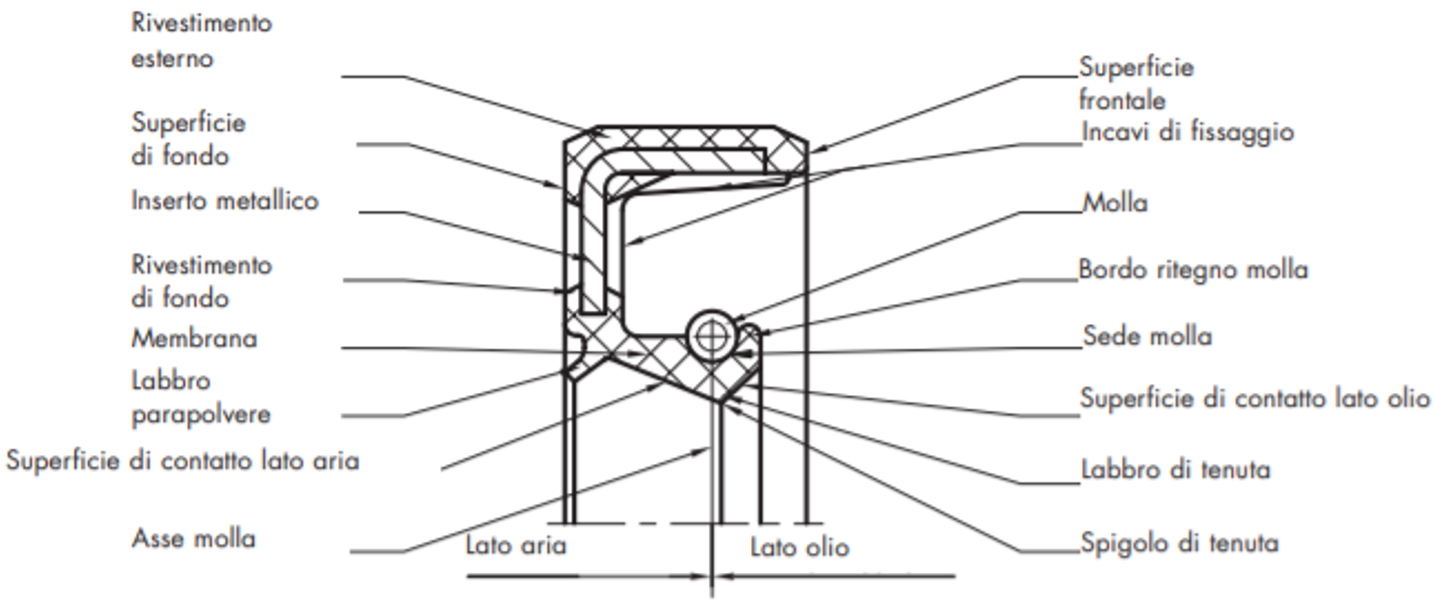
\includegraphics[scale=0.5]{Immagini/SchemaParaolio.png}
    \caption{Nomenclatura caratteristica del paraolio}
    \label{fig:SchemaParaolio}
\end{figure}

La superficie esterna garantisce una tenuta statica sicura e fissa l'anello nella sua sede. Il rivestimento esterno può essere sia in elastomero che in materiale metallico. L'inserto metallico fornisce all’anello di tenuta la stabilità necessaria, mentre l labbro di tenuta è pretensionato per mezzo di una molla che assicura la pressione del labbro sull'albero. \\
Su richiesta, si può usare un labbro parapolvere per impedire allo sporco o alla polvere di entrare all'interno del carter.\\
Gli anelli di tenuta sono conformi alla norma DIN 3760. \\
\\
\emph{Funzionamento}\\
Il contatto tra lo spigolo di tenuta del paraolio e l’albero è garantito dalla molla e dal sottodimensionamento del diametro interno del labbro di tenuta, per fare in modo che vi sia la necessaria interferenza e forza tra i due. Dopo un breve periodo di funzionamento lo spigolo di tenuta si deforma, permettendo la creazione di una sottile pellicola di fluido tra albero e spigolo, impedendo così il contatto diretto tra albero e anello, garantendone lubrificazione e durata. \\
Lo spessore di questa pellicola è compreso tra 1 e 3 micron e sul lato esterno è delimitata da un menisco, la cui tensione superficiale impedisce perdite.
\newpage
\begin{figure}[h]
    \centering
    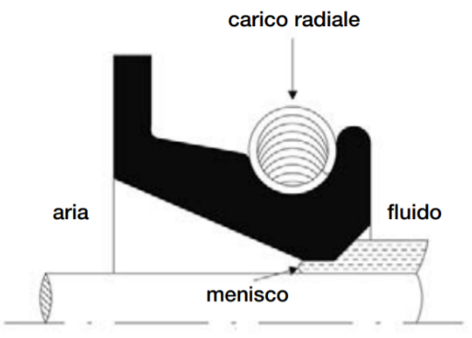
\includegraphics[scale=0.6]{Immagini/FunzionamentoParaolio1.png}
    \caption{Schema di funzionamento della tenuta}
    \label{fig:FunzionamentoParaolio1}
\end{figure}

Il compito della superficie esterna dell'anello di tenuta è di assicurare la tenuta statica nella sede di alloggiamento, ovvero impedire il passaggio del fluido tra anello e sede in tutte le possibili condizioni di funzionamento. 

\begin{figure}[h]
    \centering
    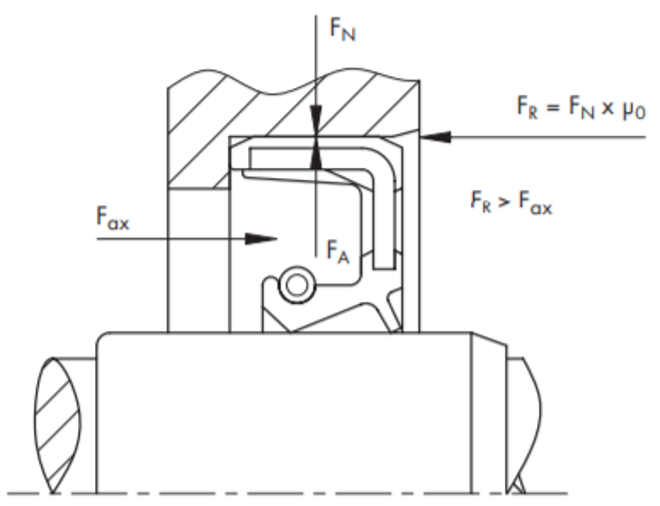
\includegraphics[scale=0.6]{Immagini/FunzionamentoParaolio2.png}
    \caption{Schema di funzionamento della tenuta}
    \label{fig:FunzionamentoParaolio2}
\end{figure}

Inoltre, alla superficie esterna della tenuta è richiesto di assolvere altri compiti:
\begin{itemize}
    \item Guida e fissaggio dell'anello di tenuta nella sede. Un fissaggio sicuro è garantito quando la forza di attrito $F_R$ risulta maggiore delle forze assiali $F_{ax}$ che vengono ad agire sull'anello di tenuta;
    \item Semplificazione delle operazioni di installazione (prevedendo smussi e raccordi);
    \item Compensazione di giochi risultanti dai differenti coefficienti di dilatazione termica. 
\end{itemize}

La scelta della corretta superficie esterna per un anello di tenuta dipende dall'applicazione specifica e dalle condizioni di funzionamento principali.\\
\newpage
Le tenute rotanti sono state inserite solamente dove necessarie, ovvero sugli alberi di
input, di output e albero 2. In particolare, il posizionamento delle tenute è visibile dal modello CAD bidimensionale del riduttore nella figura sottostante.
\begin{figure}[h]
    \centering
    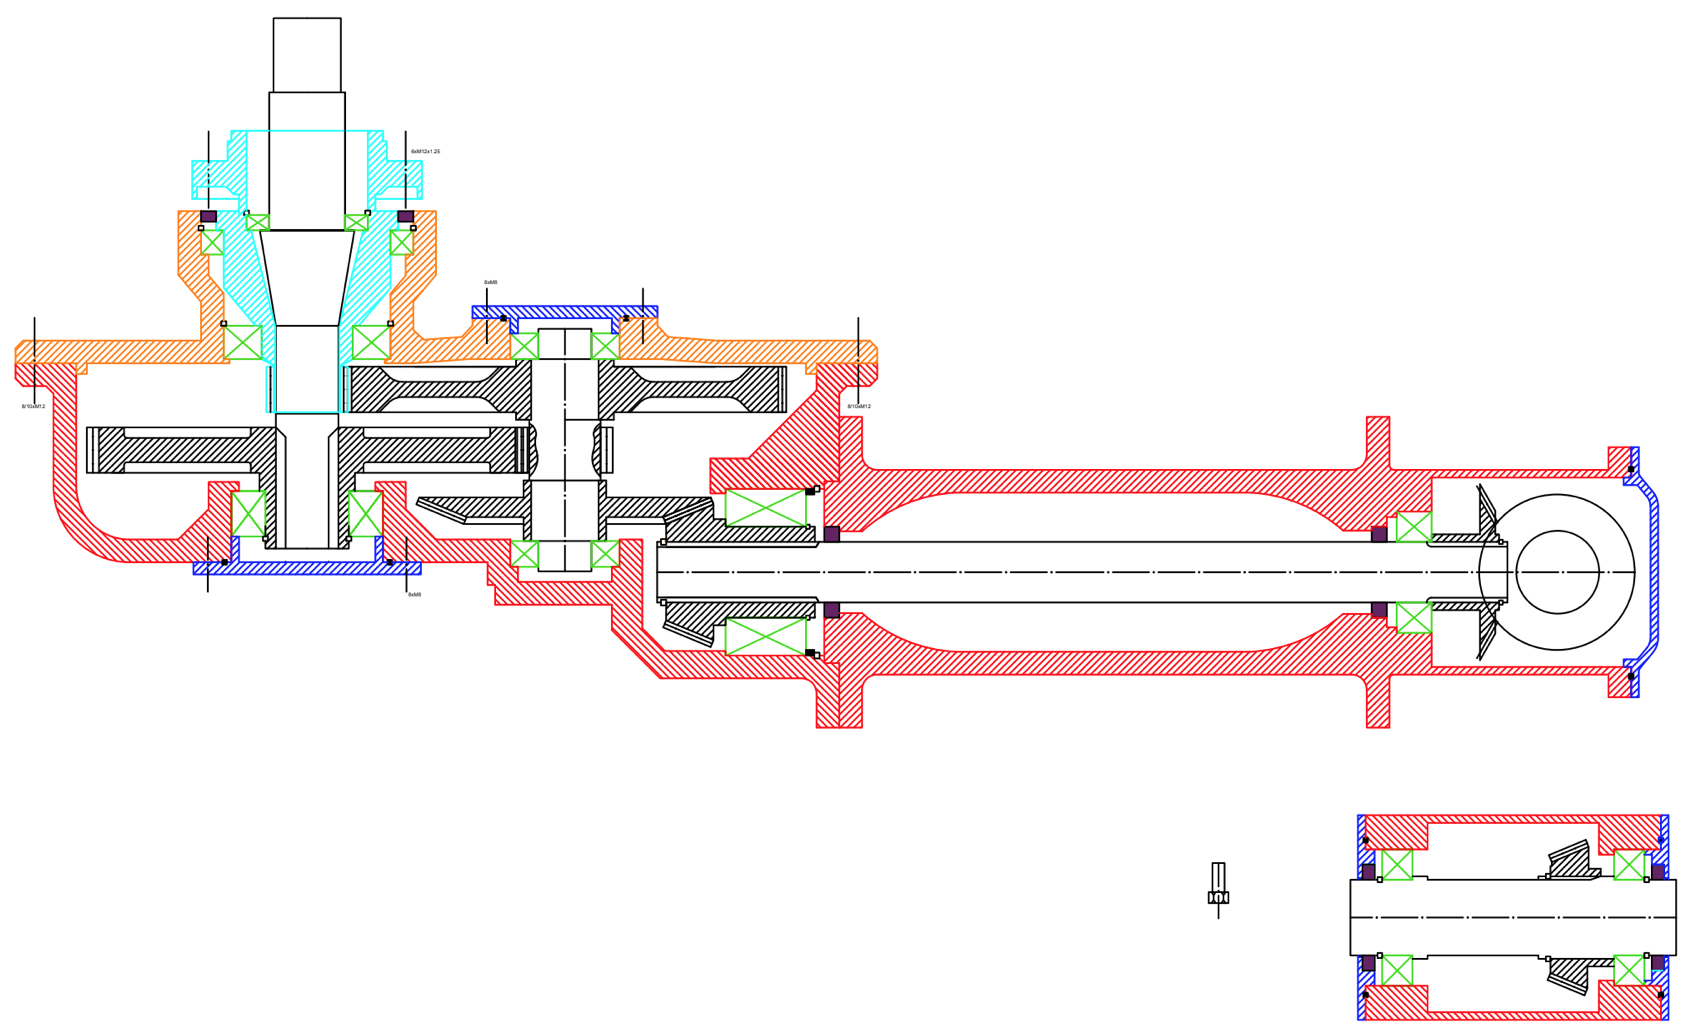
\includegraphics[scale=0.5]{Immagini/Riduttore2D.png} %IMMAGINE DA CAMBIARE, METTERE ENFASI (MAGARI CAMBIANDO COLORE O CERCHIANDO, ....) SUL POSIZIONAMENTO DEI PARAOLI
    \caption{Rappresentazione 2D del riduttore}
    \label{fig:Riduttore2D}
\end{figure}

Per il progetto sono stati scelti degli anelli di tenuta per alberi rotanti, presi dal catalogo SKF.
\newpage
\paragraph{Albero 1}
Per questo albero è stata utilizzata la tuenuta 60X70X07 CRS1 R

\begin{figure}[h]
    \centering
    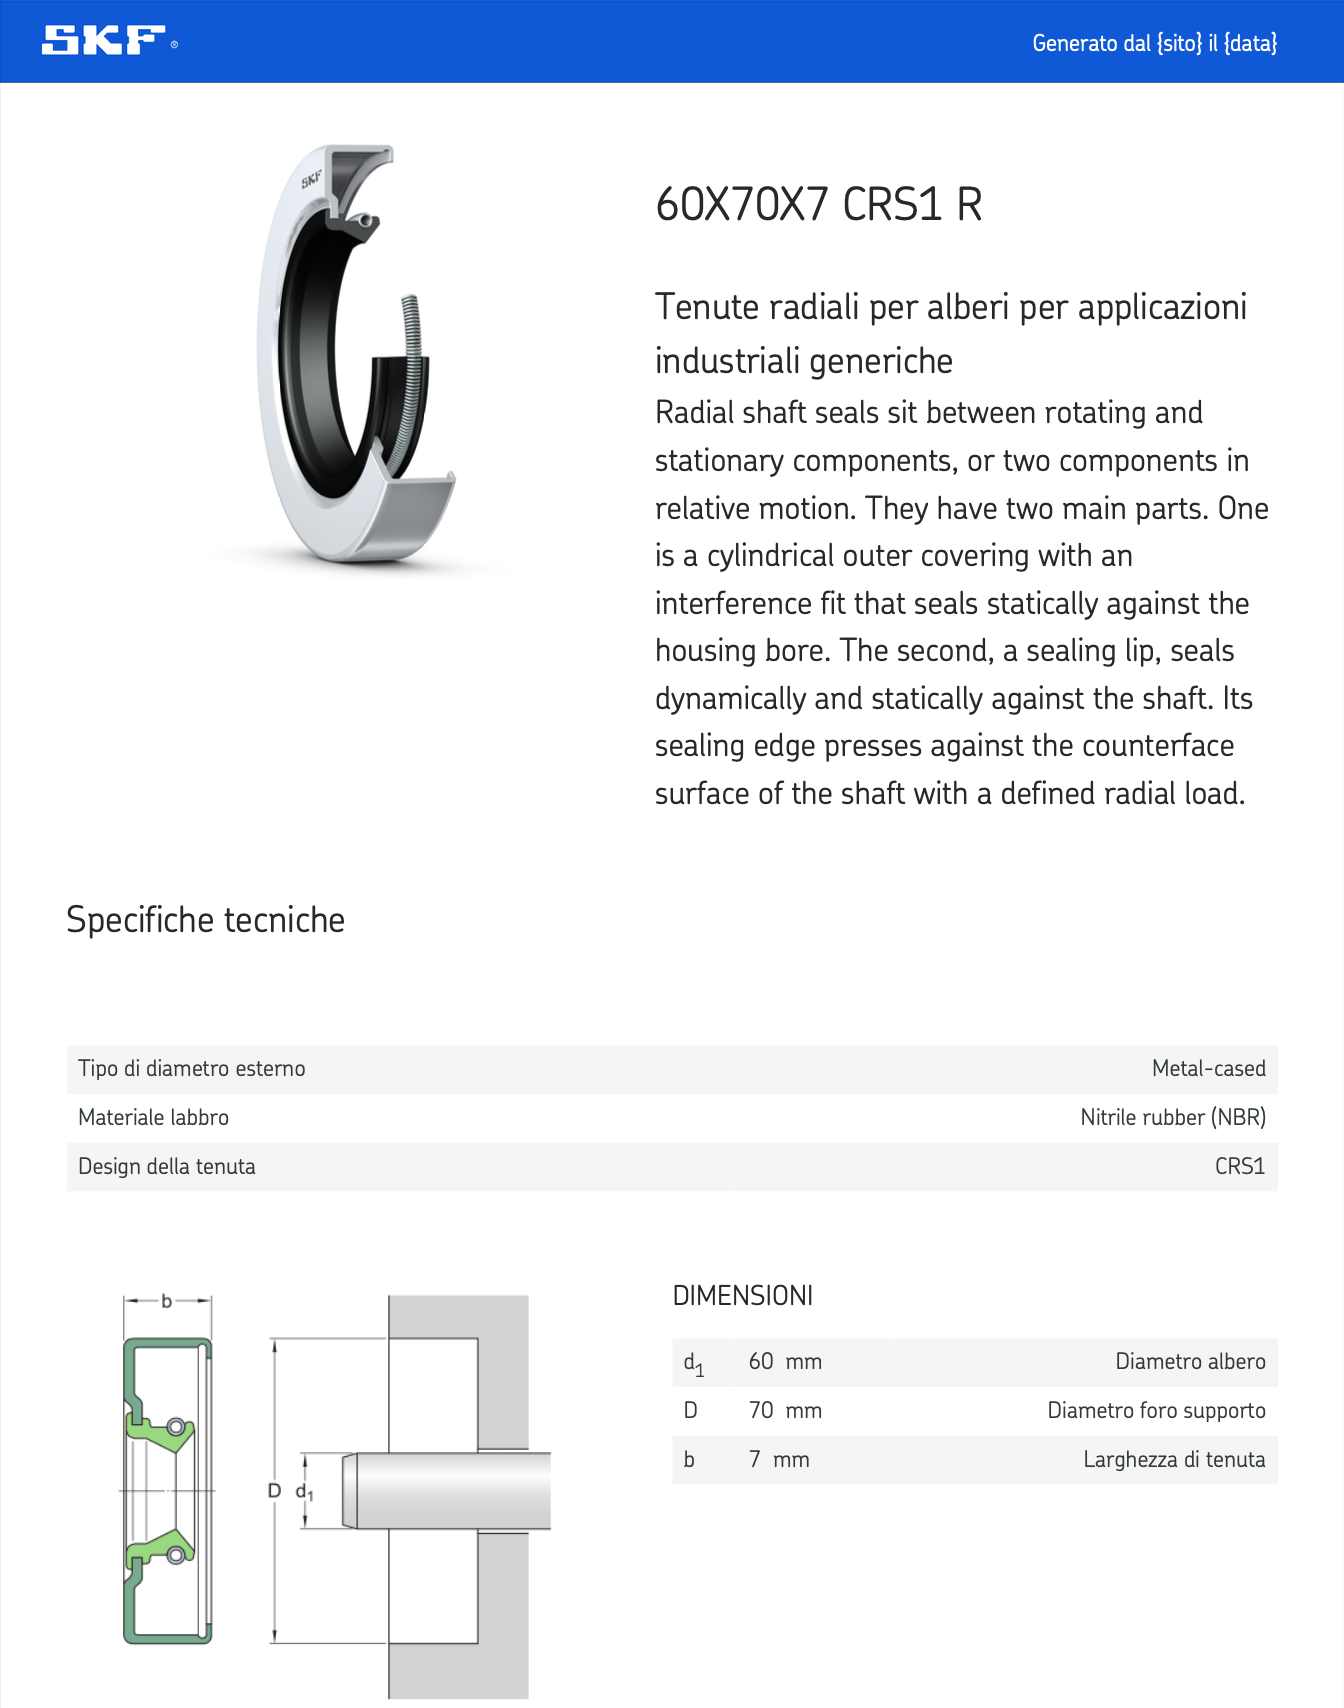
\includegraphics[scale=0.5]{Immagini/Paraolio1Albero1.png}
    \caption{Caratteristiche tecniche dei paraoli montati sull'albero 1}
    \label{fig:Paraolio1Albero1}
\end{figure}
\newpage
\begin{figure}[h]
    \centering
    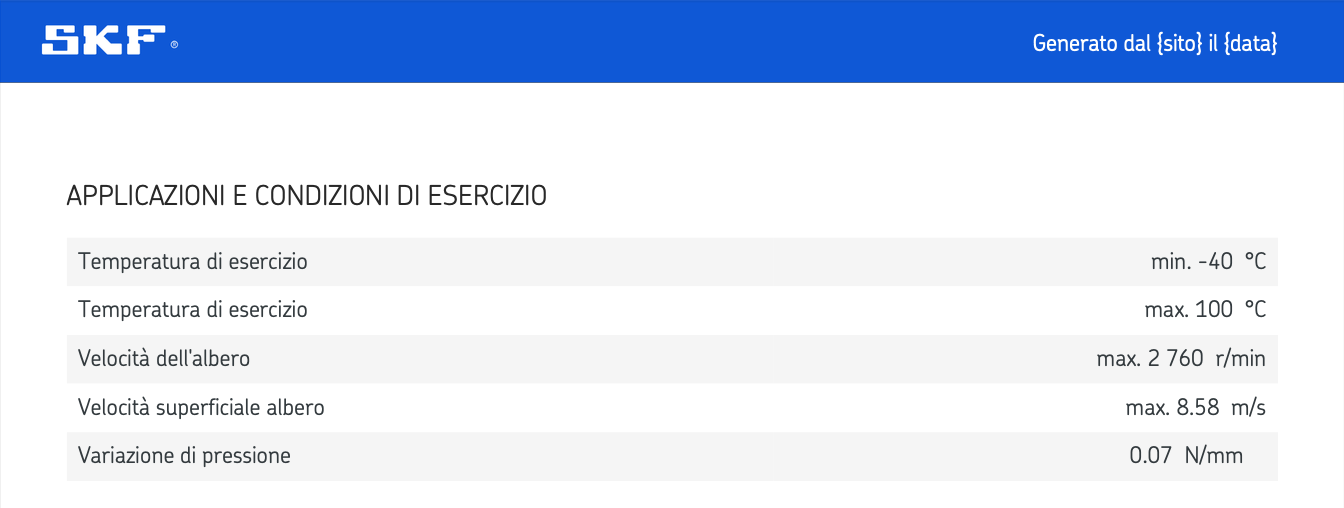
\includegraphics[scale=0.5]{Immagini/Paraolio2Albero1.png}
    \caption{Caratteristiche tecniche dei paraoli montati sull'albero 1}
    \label{fig:Paraolio2Albero1}
\end{figure}

\newpage

\paragraph{Albero 2}
Per questo albero è stata utilizzata la tenuta 40X60X10 HMS5 V.\\

\begin{figure}[h]
    \centering
    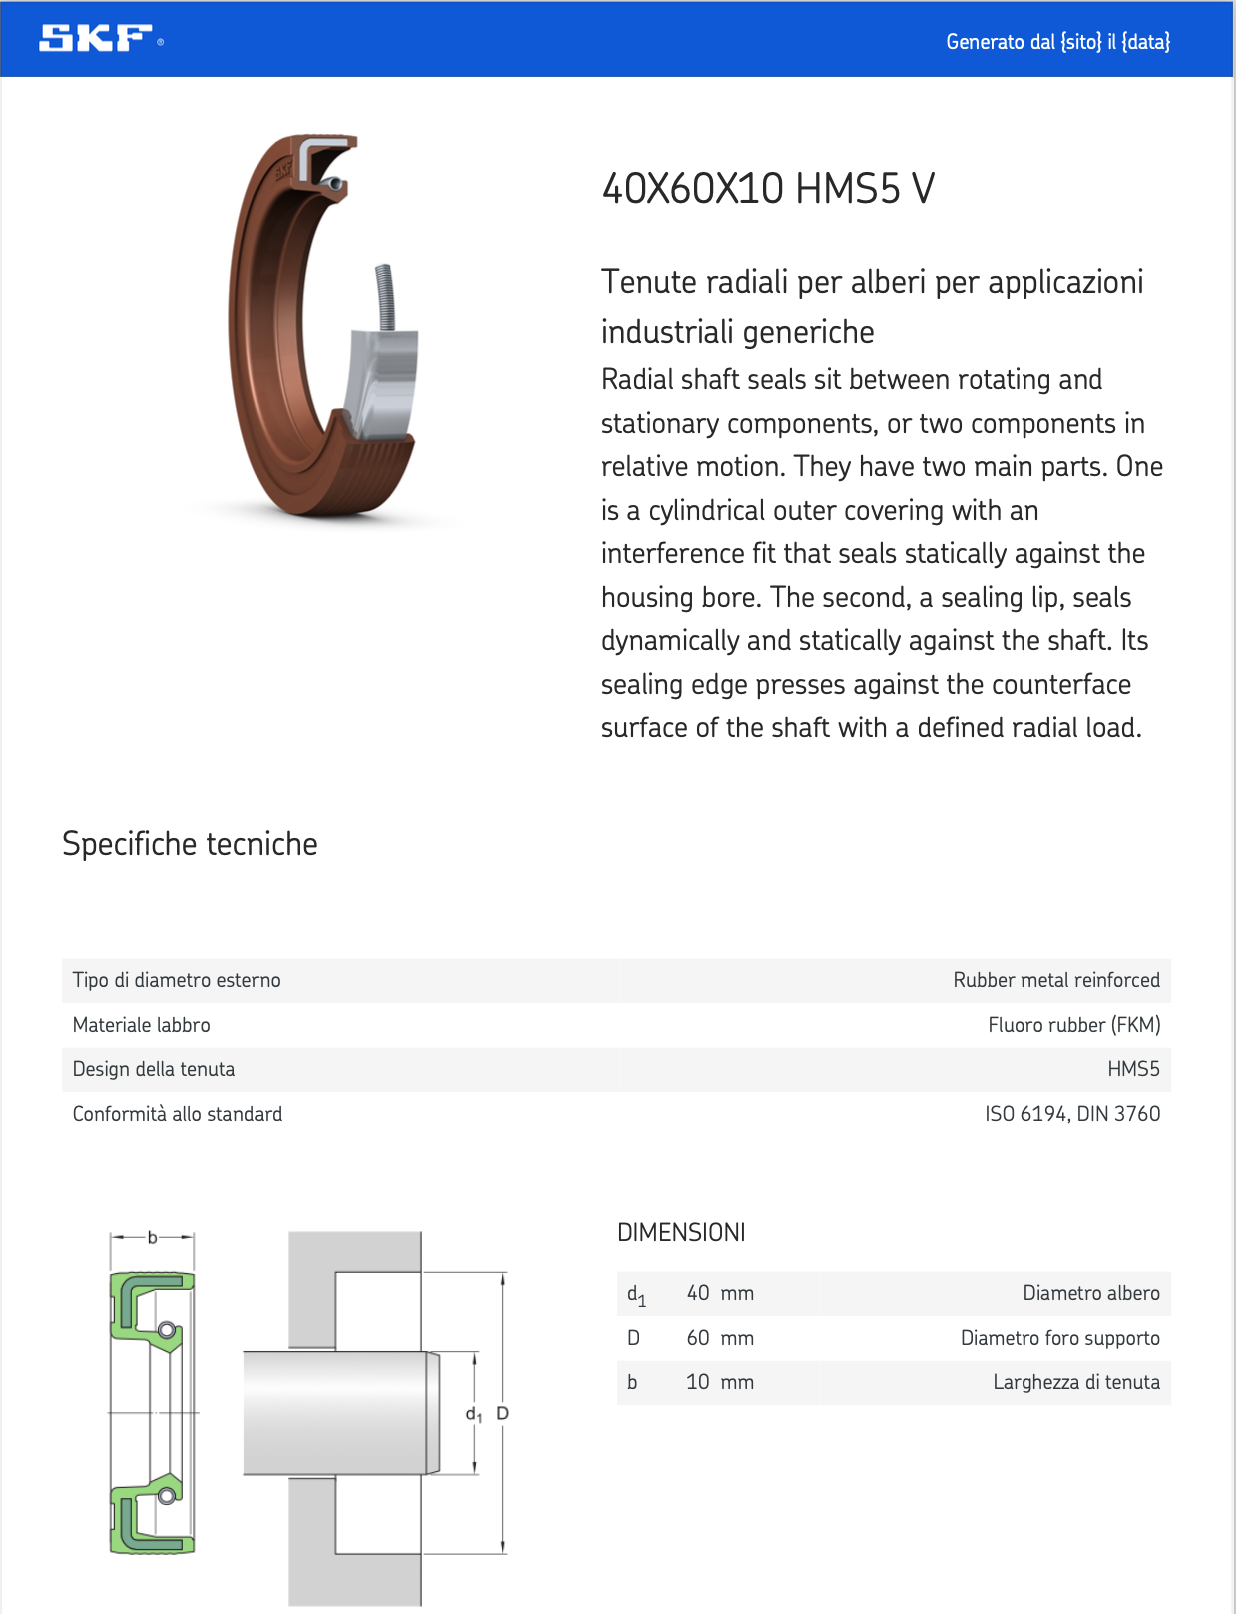
\includegraphics[scale=0.5]{Immagini/Paraolio1Albero2}
    \caption{Caratteristiche tecniche dei paraoli montati sull'albero 2}
    \label{fig:Paraolio1Albero2}
\end{figure}
\newpage
\begin{figure}[h]
    \centering
    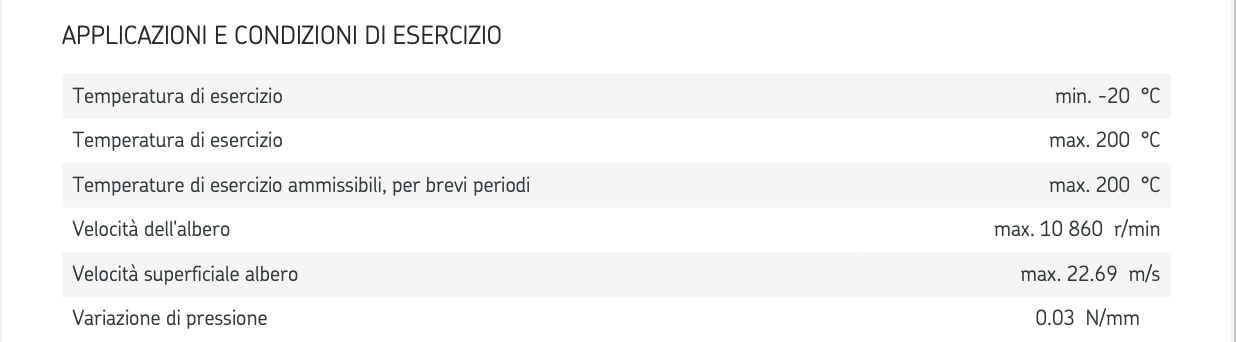
\includegraphics[scale=0.5]{Immagini/Paraolio2Albero2}
    \caption{Caratteristiche tecniche dei paraoli montati sull'albero 2}
    \label{fig:Paraolio2Albero2}
\end{figure}
\newpage
\paragraph{Albero 5}
Per questo albero è stata utilizzata la tenuta 120X140X12 HMSA10 RG.\\
\begin{figure}[h]
    \centering
    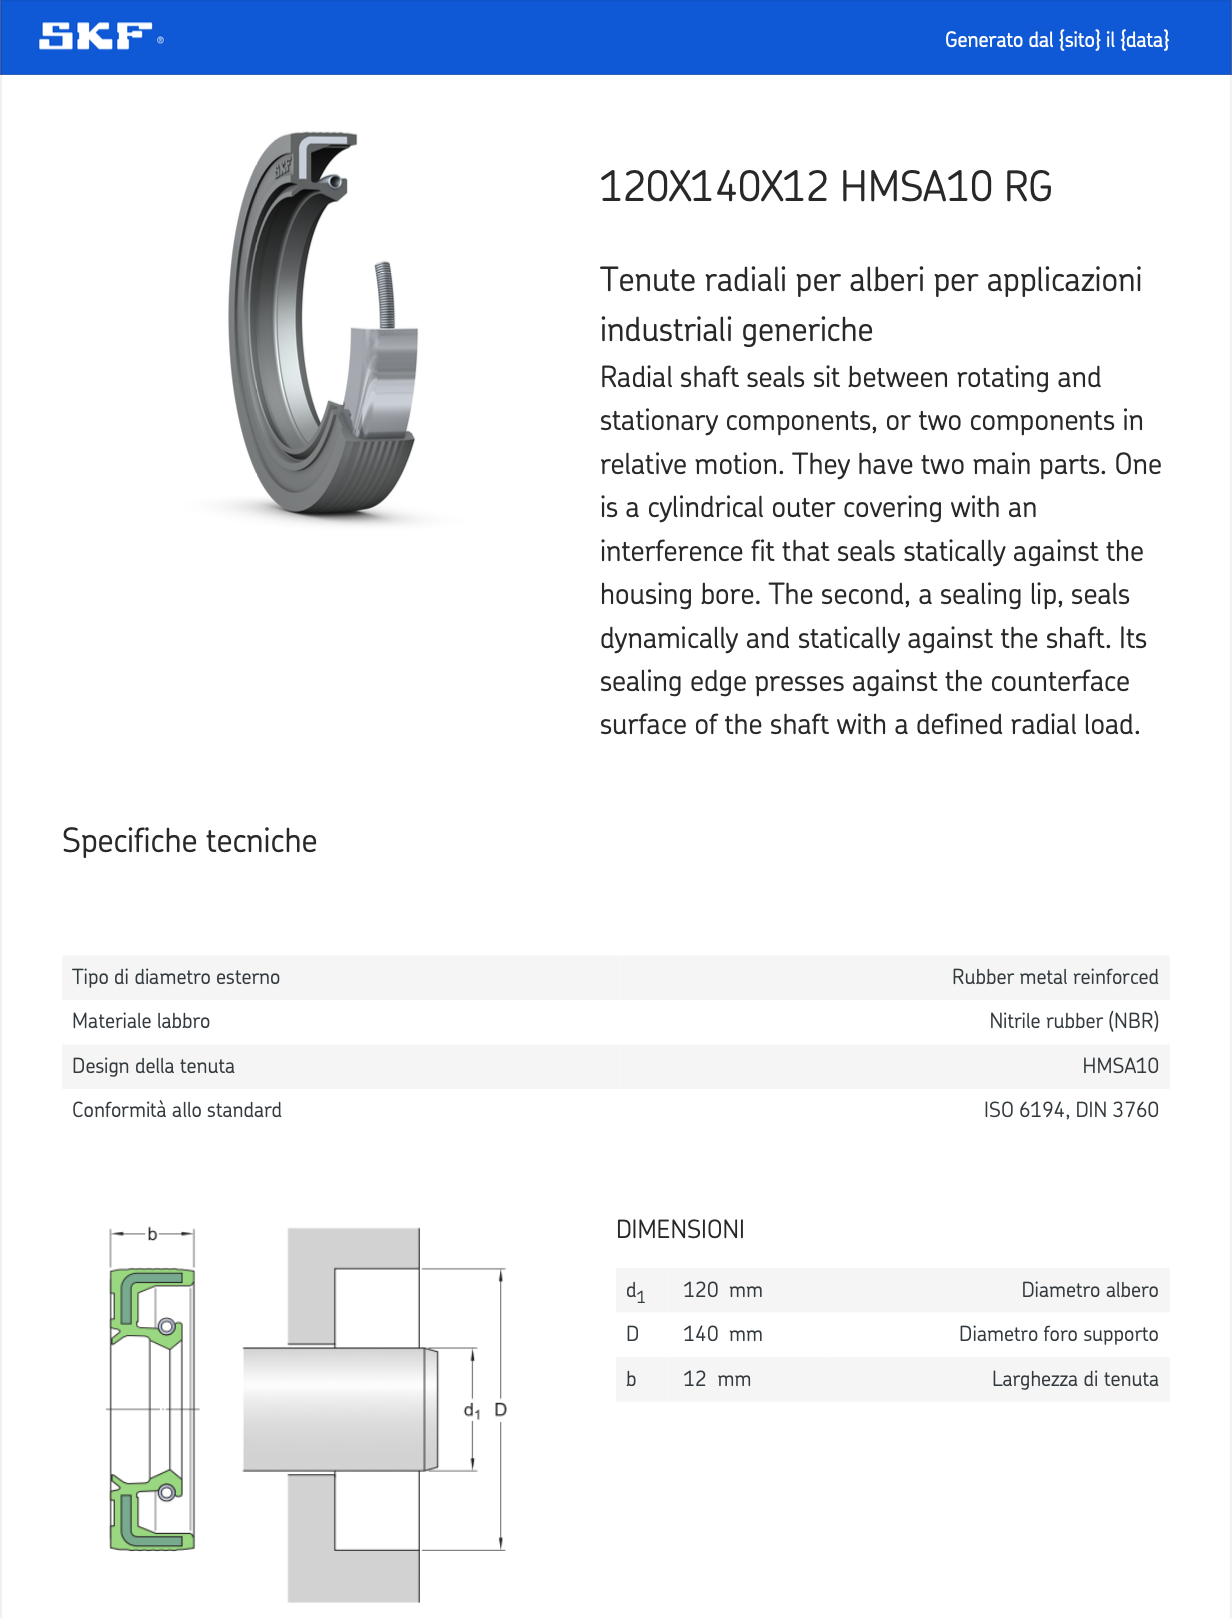
\includegraphics[scale=0.5]{Immagini/Paraolio1Albero5}
    \caption{Caratteristiche tecniche dei paraoli montati sull'albero 5}
    \label{fig:Paraolio1Albero5}
\end{figure}
\newpage
\begin{figure}[h]
    \centering
    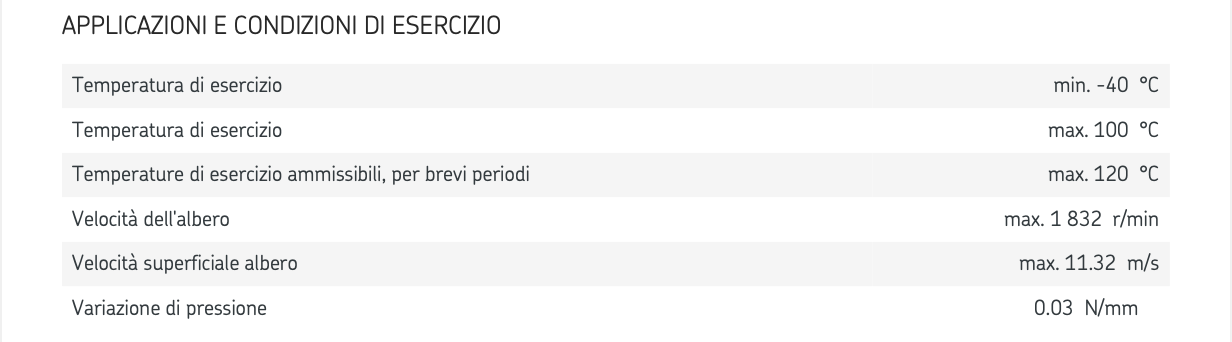
\includegraphics[scale=0.5]{Immagini/Paraolio2Albero5}
    \caption{Caratteristiche tecniche dei paraoli montati sull'albero 5}
    \label{fig:Paraolio2Albero5}
\end{figure}